\documentclass[11pt,letterpaper]{article}

% Professional packages and setup
\usepackage[utf8]{inputenc}
\usepackage[T1]{fontenc}
\usepackage{lmodern}
\usepackage{microtype}

% Colors - Professional palette
\usepackage{xcolor}
\definecolor{primaryBlue}{RGB}{25, 55, 135}
\definecolor{accentBlue}{RGB}{51, 77, 167}
\definecolor{darkGray}{RGB}{64, 64, 64}
\definecolor{mediumGray}{RGB}{96, 96, 96}
\definecolor{lightGray}{RGB}{224, 224, 224}
\definecolor{offWhite}{RGB}{248, 248, 248}

% Page layout
\usepackage[letterpaper, margin=0.65in, top=0.5in, bottom=0.6in]{geometry}
\usepackage{setspace}
\setstretch{1.0}

% Graphics and design
\usepackage{tikz}
\usepackage{graphicx}
\usepackage{fontawesome5}
\usetikzlibrary{positioning,shapes,backgrounds}

% Typography and formatting
\usepackage[scaled=0.85]{helvet}
\renewcommand\familydefault{\sfdefault}
\usepackage{titlesec}
\usepackage{enumitem}
\usepackage{tabularx}
\usepackage{array}

% Hyperlinks
\usepackage[hidelinks]{hyperref}
\hypersetup{
    colorlinks=true,
    linkcolor=primaryBlue,
    urlcolor=primaryBlue,
    citecolor=primaryBlue
}

% No page numbers
\pagestyle{empty}

% Custom commands
\newcommand{\sectionline}{\noindent\textcolor{primaryBlue}{\rule{\textwidth}{1.5pt}}}
\newcommand{\subsectionline}{\noindent\textcolor{lightGray}{\rule{\textwidth}{0.5pt}}}

% Section formatting
\titleformat{\section}
{\Large\bfseries\color{primaryBlue}}
{}
{0em}
{\MakeUppercase}[\vspace{1pt}\sectionline\vspace{3pt}]

\titlespacing*{\section}{0pt}{8pt}{4pt}

% Professional entry formatting
\newcommand{\profentry}[4]{
    \begin{tabularx}{\textwidth}{@{}X r@{}}
        \textbf{\color{darkGray}#1} & \textcolor{mediumGray}{\textit{#2}} \\
        \textcolor{mediumGray}{#3} & #4
    \end{tabularx}
}

\newcommand{\listentry}[1]{
    \item[\textcolor{accentBlue}{\small\faAngleRight}] #1
}

% Custom lists
\setlist[itemize]{leftmargin=12pt, itemsep=1pt, parsep=0pt, topsep=2pt}

% Header command
\newcommand{\makeheader}{
\begin{center}
\begin{tikzpicture}[remember picture, overlay]
    \fill[primaryBlue!8] (-0.5\paperwidth,-0.8) rectangle (0.5\paperwidth,1.2);
\end{tikzpicture}
\vspace{3pt}
{\fontsize{26}{30}\selectfont\bfseries\color{primaryBlue}JORGE J. ORTIZ}\\[2pt]
{\Large\color{darkGray}Associate Professor (with Tenure)}\\[1pt]
{\large\color{mediumGray}Electrical and Computer Engineering \textbullet\ Director, Sensing and Reasoning Lab}\\[1pt]
{\large\bfseries\color{darkGray}Rutgers University}\\[4pt]

\begin{tikzpicture}
\node[fill=primaryBlue!10, rounded corners=12pt, inner sep=6pt] {
\begin{tabular}{c@{\hspace{12pt}}c@{\hspace{12pt}}c}
\faEnvelope\ \href{mailto:jorge.ortiz@rutgers.edu}{\color{primaryBlue}{jorge.ortiz@rutgers.edu}} &
\faGlobe\ \href{http://jorgeortizphd.info}{\color{primaryBlue}{jorgeortizphd.info}} &
\faPhone\ \color{darkGray}{617-784-6550}
\end{tabular}
};
\end{tikzpicture}
\end{center}
\vspace{2pt}
}

\begin{document}

\makeheader

\section{Education}
\profentry{Ph.D., Computer Science}{2013}{University of California, Berkeley}{}\\[2pt]
\profentry{M.S., Computer Science}{2010}{University of California, Berkeley}{}\\[2pt]
\profentry{B.S., Computer Science}{2003}{Massachusetts Institute of Technology}{}

\section{Academic Experience}
\profentry{Associate Professor (with Tenure)}{Sept. 2025 -- Present}{Rutgers University, Electrical and Computer Engineering}{}\\[2pt]
\profentry{Assistant Professor}{Sept. 2018 -- 2025}{Rutgers University, Electrical and Computer Engineering}{}\\[2pt]
\profentry{Director, Sensing and Reasoning (SnR) Lab}{Sept. 2018 -- Present}{Rutgers University}{}

\section{Industry Leadership}
\profentry{AI \& Computer Vision Lead, Baseball Operations}{Dec. 2019 -- Present}{New York Yankees}{}\\[2pt]
\profentry{Research Staff Member}{Dec. 2013 -- Aug. 2018}{IBM Research}{}

\vspace{2pt}
\begin{center}
\textcolor{mediumGray}{\rule{0.8\textwidth}{0.5pt}}
\end{center}
\vspace{2pt}

\section{Research Expertise}
\begin{center}
\begin{tikzpicture}
\node[fill=offWhite, rounded corners=8pt, inner sep=10pt, text width=\textwidth-20pt, align=center] {
\textbf{\color{primaryBlue}Multimodal Learning \& AI} \textbullet\ 
\textbf{\color{primaryBlue}Human-Computer Interaction} \textbullet\ 
\textbf{\color{primaryBlue}IoT \& Smart Environments}\\[2pt]
\textbf{\color{primaryBlue}Computer Vision \& Sensing} \textbullet\ 
\textbf{\color{primaryBlue}Machine Learning Applications}
};
\end{tikzpicture}
\end{center}

\section{Key Achievements \& Recognition}
\begin{itemize}
\listentry{\textbf{\color{primaryBlue}Judge}, Newsweek AI Impact Awards 2025}
\listentry{\textbf{\color{primaryBlue}Keynote Speaker}, IEEE SECON Workshop on Smart and Connected Indoor Environments (2017)}
\listentry{\textbf{\color{primaryBlue}Best Paper Awards \& Finalists}: ICISSP 2018 (Award), IoTDI 2019 (Finalist), BuildSys 2015 (2× Finalist)}
\listentry{\textbf{\color{primaryBlue}Distinguished Panels}: JPMC Hispanic Heritage Month, Columbia Sports \& AI Symposium}
\listentry{NSF Graduate Fellowship Honorable Mention, Qualcomm Innovation Fellowship Finalist}
\end{itemize}

\section{Research Funding (\$6.9M+ Total)}
\begin{itemize}
\listentry{\textbf{\color{primaryBlue}NSF ReDDDoT Phase 2}: Leveraging Urban AI in Harlem, Co-PI \textbf{(\$1.45M)}}
\listentry{\textbf{\color{primaryBlue}NIH CAMERA Platform}: Context-Aware Multimodal Research Platform, Co-PI \textbf{(\$1.08M)}}
\listentry{\textbf{\color{primaryBlue}NSF Engineering Research Center}: Smart Streetscapes, Site PI \textbf{(\$2.3M)} Rutgers}
\listentry{\textbf{\color{primaryBlue}NSF IUCRC}: Standards and Ethics in Artificial Intelligence, PI \textbf{(\$20K)}}
\end{itemize}

\section{Selected Publications}
\begin{itemize}
\listentry{\textbf{J. Ortiz} et al., ``DeviceMien: Network Device Behavior Modeling for Identifying Unknown IoT Devices,'' \textit{ACM IoTDI}, 2019. \textbf{\color{accentBlue}[Best Paper Finalist]}}

\listentry{Y. Sun, N. Salami Pargoo, P. Jin, \textbf{J. Ortiz}, ``Optimizing Autonomous Driving for Safety: A Human-Centric Approach with LLM-Enhanced RLHF,'' \textit{ACM UbiComp Companion}, 2024.}

\listentry{M. Aldeer, \textbf{J. Ortiz}, et al., ``PatientSense: Patient Discrimination from in-Bottle Sensors Data,'' \textit{ACM MobiQuitous}, 2019.}

\listentry{Z. Hussain et al., ``Non-Invasive Techniques for Monitoring Different Aspects of Sleep: A Comprehensive Review,'' \textit{ACM Trans. Computing for Healthcare}, 2022.}

\listentry{D. Hong, H. Wang, \textbf{J. Ortiz}, K. Whitehouse, ``The Building Adapter: Towards Quickly Applying Building Analytics at Scale,'' \textit{ACM BuildSys}, 2015. \textbf{\color{accentBlue}[Best Paper Finalist]}}
\end{itemize}

\section{Leadership \& Service}
\begin{itemize}
\listentry{\textbf{\color{primaryBlue}Conference Leadership}: Steering Committee Chair BuildSys (2024-25), General Chair BuildSys (2022)}
\listentry{\textbf{\color{primaryBlue}2025 Technical Program Committees}: ACM MobiHoc, Sensys, BuildSys, ICLR}
\listentry{\textbf{\color{primaryBlue}Workshop Organization}: NeurIPS 2021 Deep Learning \& Differential Equations (Organizer)}
\listentry{\textbf{\color{primaryBlue}Major Conference Roles}: CPS-IoT Week 2019 Publication Chair (5 conferences)}
\end{itemize}

\section{Mentoring \& Students}
\textbf{\color{primaryBlue}Ph.D. Graduates}: Tahiya Chowdhury (2022), Murtadha Aldeer (2023), Tong Wu (2023)\\[2pt]
\textbf{\color{primaryBlue}Research Focus}: Human activity sensing, multimodal learning, IoT behavior understanding

\vspace{4pt}
\begin{center}
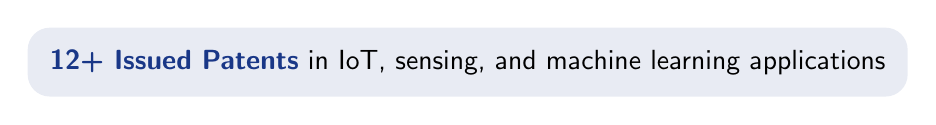
\begin{tikzpicture}
\node[fill=primaryBlue!10, rounded corners=8pt, inner sep=8pt] {
\textbf{\color{primaryBlue}12+ Issued Patents} in IoT, sensing, and machine learning applications
};
\end{tikzpicture}
\end{center}

\end{document} 